\documentclass[11pt]{article}
\usepackage[margin=1in]{geometry}
\usepackage{microtype}
\usepackage{hyperref}
\usepackage{titlesec}
\usepackage{enumitem}
\usepackage{graphicx}
\usepackage{tikz}
\usepackage{listings}
\usepackage{xcolor}

\hypersetup{
  colorlinks=true,
  linkcolor=blue,
  urlcolor=blue,
  citecolor=blue,
  pdfauthor={Ankit Malhotra},
  pdftitle={CRIITS: A Transaction-Agnostic State Machine},
}

\titleformat{\section}[block]{\large\bfseries}{--}{0pt}{}
\titleformat{\subsection}[block]{\normalsize\bfseries}{--}{0pt}{}

\lstdefinelanguage{json}{
    basicstyle=\ttfamily\small,
    numbers=left,
    numberstyle=\tiny,
    stepnumber=1,
    numbersep=5pt,
    showstringspaces=false,
    breaklines=true,
    frame=single,
}
\lstset{
  basicstyle=\ttfamily\small,
  frame=single,
  breaklines=true,
  showstringspaces=false
}

\begin{document}
\begin{titlepage}
\centering
\vspace*{1cm}
{\Huge \textbf{CRIITS}}\par
\vspace{0.4cm}
{\Large A Transaction-Agnostic State Machine for Reliable End-to-End Processing}\par
\vspace{1.5cm}
{\large \textbf{Author:} Ankit Malhotra}\par
\vspace{0.2cm}
Version 1.0 \quad | \quad Date: 16 September 2025\par
\vfill
\begin{tabular}{p{0.9\textwidth}}
\textbf{Abstract}\\[0.2cm]
Modern transactional systems span multiple services and networks. Failures, retries, and out-of-order delivery make it hard to guarantee that no transaction is missed. CRIITS defines four canonical phases—CR (Created), I (Initiated), I (0..n Intermediary), and TS (Terminal State)—plus operating invariants, a reference architecture, and a polling \& reconciliation strategy to deliver observability and finality across domains.\\[0.3cm]
\textbf{License}: CC BY 4.0 \quad \textbar\  \textbf{Contact}: \href{mailto:connect@ankitmalhotra.com}{connect@ankitmalhotra.com} \quad \textbar\  
\textbf{DOI}: \href{https://doi.org/10.5281/zenodo.17132329}{10.5281/zenodo.17132329}
\end{tabular}
\vfill
\end{titlepage}

\tableofcontents
\newpage

\section{Introduction}
Distributed systems push business logic across APIs, queues, databases, and third-party gateways. Each hop introduces places to lose context or double-act on messages. Patterns like Sagas, Event Sourcing, and CQRS help, but teams still reinvent status semantics and pollers per use case.
CRIITS proposes a small, standard state machine and operating convention to unify tracking, bound failure handling, and make “missed transaction” a measurable, alertable condition—remaining agnostic to domain (payments, KYC, logistics, content moderation, etc.).

\section{The CRIITS Model}
\subsection{Canonical States}
\begin{itemize}[leftmargin=*]
\item \textbf{CR — Created}: Transaction accepted by the system of record (SOR). ID minted, minimal validation passed, persistence guaranteed.
\item \textbf{I — Initiated}: Execution has started (request sent to downstream or workflow engaged).
\item \textbf{I — Intermediary (0..n)}: Checkpoints representing externally verifiable progress (e.g., 3-DS required, vendor acknowledged, shipment picked).
\item \textbf{TS — Terminal State}: Finality with mutually exclusive outcomes: TS.SUCCEEDED, TS.FAILED, TS.CANCELED, TS.EXPIRED.
\end{itemize}

\subsection{Invariants}
\begin{enumerate}[leftmargin=*]
\item \textbf{Monotonicity}: forward-only transitions CR $\to$ I $\to$ I* $\to$ TS.
\item \textbf{Completeness}: every transaction eventually reaches a single TS.
\item \textbf{Idempotency}: replaying the same transition is safe.
\item \textbf{Auditability}: transitions are append-only with causality metadata.
\end{enumerate}

\subsection{State Machine Diagram}
\begin{figure}[h]
\centering
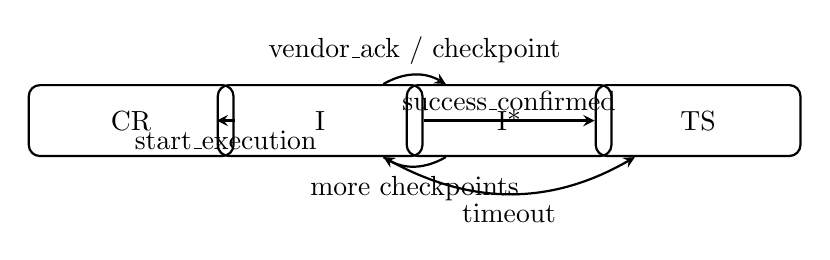
\begin{tikzpicture}[node distance=2.4cm, >=stealth, thick, auto]
\tikzstyle{state}=[rectangle, rounded corners, draw, minimum width=2.6cm, minimum height=0.9cm]
\node[state] (cr) {CR};
\node[state, right of=cr] (i) {I};
\node[state, right of=i] (istar) {I*};
\node[state, right of=istar] (ts) {TS};
\path[->] (cr) edge node {start\_execution} (i);
\path[->] (i) edge[bend left] node {vendor\_ack / checkpoint} (istar);
\path[->] (istar) edge[bend left] node {more checkpoints} (i);
\path[->] (i) edge node {success\_confirmed} (ts);
\path[->] (i) edge[bend right] node[below] {timeout} (ts);
\end{tikzpicture}
\caption{CRIITS canonical state progression with example events.}
\end{figure}

\section{Reference Architecture}
Core components: Transaction Gateway, Orchestrator/Workers, Append-only Event Log, State Projection, Dispatchers (webhook emitter + outbox), Poller/Reconciler, Dead-Letter \& Triage.

\subsection{Component Diagram}
\begin{figure}[h]
\centering
\begin{tikzpicture}[node distance=1.8cm, >=stealth, thick, auto]
\tikzstyle{box}=[rectangle, draw, rounded corners, minimum width=3.4cm, minimum height=1cm]
\node[box] (client) {Clients / Producers};
\node[box, right=of client] (tg) {Transaction Gateway};
\node[box, right=of tg] (elog) {Append-only Event Log};
\node[box, below=of elog] (proj) {State Projection (tx\_head)};
\node[box, below=of tg] (orch) {Orchestrator / Workers};
\node[box, right=of elog, xshift=3.6cm] (ext) {External Vendors};
\node[box, below=of proj] (poll) {Poller / Reconciler};
\node[box, below=of orch] (dlq) {Dead-Letter \& Triage};
\path[->] (client) edge (tg);
\path[->] (tg) edge node {CR} (elog);
\path[->] (orch) edge[bend left] node {I/TS events} (elog);
\path[->] (elog) edge (proj);
\path[->] (proj) edge (poll);
\path[->] (orch) edge (dlq);
\path[->] (orch) edge[bend left] node {Idempotent calls} (ext);
\path[->] (poll) edge[bend left] node {Reconcile} (ext);
\end{tikzpicture}
\caption{Reference architecture for CRIITS deployment.}
\end{figure}

\section{Implementation Guide}
\subsection{Minimal Data Model (SQL)}
\lstinputlisting[language=SQL]{sql/ddl.sql}

\subsection{REST Interface (Sketch)}
\begin{lstlisting}[language=]
POST /transactions           -> returns tid (CR recorded)
POST /transactions/{tid}/events  -> advances state (idempotency_key required)
GET  /transactions/{tid}     -> current state + timeline
GET  /transactions?state!=TS.*&stalled_gt=5m  -> for poller
\end{lstlisting}

\subsection{Polling \& Reconciliation}
Adaptive backoff: immediately after I, poll at 10s cadence; after 5 minutes, widen to 30s; after 30 minutes, 2m; cap at 10m. Reset cadence upon any new event.
Reconciliation loop periodically ingests authoritative lists from vendors (e.g., settlement files, KYC batches) and writes missing I/TS events retroactively with observed timestamps from evidence.

\subsection{Idempotency \& Concurrency}
Producer rule: reuse the same idempotency key for a logical effect. Consumer rule: de-dupe on idempotency key. Use optimistic concurrency on projection head.

\subsection{Timeouts, Retries, Escalation}
Per-state TTL; retry budgets; on exhaustion, TS.EXPIRED with reason code. Automatic ticketing for SLO breaches.

\section{Observability \& SLOs}
\subsection{Core Metrics}
Time-to-Finality (CR$\to$TS), Stalled Rate (I-state dwell beyond TTL), Missed-by-Push vs Rescued-by-Poll, Duplicate Event Rate, Transition Error Rate.
\subsection{Dashboards}
Funnel CR$\to$I$\to$I*$\to$TS by cohort; dwell heatmaps; top failure codes.

\section{Security, Compliance, Audit}
Data minimization and encryption; append-only log with checksums; PII/PCI segregation; retention and archiving.

\section{Case Studies (Domain-Agnostic)}
\subsection{Payment Authorization \& Capture}
CR: order created; I: auth initiated; I: 3-DS; I: AUTHORIZED; I: CAPTURE\_PENDING; TS: SUCCEEDED/FAILED/EXPIRED.
\subsection{KYC Verification}
CR: KYC submitted; I: vendor hit; I: MATCHED/MISMATCH/MANUAL\_REVIEW; TS: APPROVED/REJECTED/EXPIRED.
\subsection{Logistics Fulfilment}
CR: shipment created; I: pickup; I: in-transit; TS: DELIVERED/RTO/LOST.

\section{Adoption Playbook \& Maturity}
Level 0: map existing statuses; Level 1: emit events; Level 2: outbox + poller; Level 3: SLOs \& automated reconciliation; Level 4: vendor contracts reference CRIITS states.

\section{Limitations \& Future Work}
CRIITS standardizes observation, not business workflows; some ecosystems lack reliable reconciliation APIs. Future: reference DSL, open schemas, conformance tests.

\section{Conclusion}
Confining lifecycles to CR $\to$ I $\to$ I* $\to$ TS with strict invariants, idempotency, and push+poll recovery yields uniform observability and measurable finality with minimal disruption.

\appendix
\section{Appendix A: State \& Reason Codes}
\begin{itemize}[leftmargin=*]
\item CR
\item I.* (namespaced): I.AUTH\_REQUIRED, I.AUTHORIZED, I.CAPTURE\_PENDING
\item TS.SUCCEEDED \textbar\ TS.FAILED \textbar\ TS.CANCELED \textbar\ TS.EXPIRED
\end{itemize}
Reason codes (examples): PG\_DECLINED, TIMEOUT, INVALID\_INPUT, RETRY\_BUDGET\_EXCEEDED, DOWNSTREAM\_5XX, HUMAN\_REJECTED.

\section{Appendix B: Sample Event (JSON)}
\begin{lstlisting}[language=json]
{
  "tid": "8c2e8b3c-2e3d-4c7d-9c1a-8f07c5f2c901",
  "from_state": "I.AUTHORIZED",
  "to_state": "TS.SUCCEEDED",
  "event_type": "success_confirmed",
  "idempotency_key": "auth-8c2e8b3c-...-try-1",
  "producer": "capture-worker-v3",
  "observed_at": "2025-09-12T07:10:12Z",
  "evidence": {
    "pg_ref": "PG12345",
    "amount_minor": 129900,
    "currency": "INR",
    "files": [{"type":"settlement","uri":"s3://.../2025-09-12/settlement.csv"}]
  },
  "causation_id": "a2ff7e84-...-42",
  "correlation_id": "order-5b7..."
}
\end{lstlisting}

\section{Appendix C: Querying Stalled Transactions (SQL)}
\begin{lstlisting}[language=SQL]
SELECT tid, state, last_changed_at
FROM tx_head
WHERE state LIKE 'I.%'
  AND last_changed_at < now() - interval '15 minutes';
\end{lstlisting}

\section{Appendix D: Operator Playbook (RMG / Poker Example)}
\subsection*{Scope}
Applies CRIITS to deposits, withdrawals, KYC, table buy-ins, and game-result settlements in a real-money gaming (RMG) poker platform.

\subsection*{KPIs}
TTF (CR$\to$TS) per flow; Stalled Rate in I.AUTH\_REQUIRED, I.KYC\_REVIEW, I.CAPTURE\_PENDING; Duplicate Events per producer; Missed-by-Push vs Rescued-by-Poll.

\subsection*{Alerting}
\begin{itemize}[leftmargin=*]
\item High: Stalled Rate > 2\% for > 10 min in any I-state.
\item High: TTF P95 breach vs SLA (e.g., deposits > 2 min, withdrawals > 2 hours).
\item Medium: Duplicate Event Rate > 0.1\% over 5 min window.
\item Medium: Vendor webhook silence > 15 min; switch to aggressive polling policy.
\end{itemize}

\subsection*{Runbooks}
\textbf{Deposits}: If in I.CAPTURE\_PENDING beyond 15 min, query settlement file; on match, emit TS.SUCCEEDED with evidence; else, escalate and auto-create ticket.
\newline
\textbf{Withdrawals}: If I.MANUAL\_REVIEW beyond 24h, batch notify Risk; auto-expire to TS.EXPIRED with reason if KYC outdated.
\newline
\textbf{KYC}: If vendor mismatch in evidence, route to HUMAN\_REVIEW and enforce TS on resolution; ensure new transactions reference parent\_tid for reversals.

\subsection*{Dashboards}
Funnel per flow; Dwell heatmap by state; Failure codes by vendor; Real-time Missed-by-Push vs Rescued-by-Poll.

\section{Appendix E: References}
{\small See \texttt{references.bib} for canonical patterns: Sagas, Outbox, Event Sourcing.}

\end{document}
